\documentclass[UTF8,a4paper,11pt,fontset=fandol]{ctexart}
\newcommand{\DocTitle}{实验06：小型语言模型实现与中文古诗生成}
\newcommand{\DocSubject}{135分钟；因果注意力、字符级语言模型、中文古诗、107平台Slurm}
\newcommand{\DocShortTitle}{实验06：中文古诗生成}
\newcommand{\DocType}{学生讲义与实验手册}
% Shared style for integrated experiment handouts.
\usepackage[left=2.15cm,right=2.15cm,top=2.25cm,bottom=2.15cm,headsep=0.7cm]{geometry}
\usepackage{amsmath,amssymb}
\usepackage{booktabs,array,tabularx,longtable,multirow}
\usepackage{enumitem}
\usepackage{xcolor}
\usepackage{graphicx}
\usepackage{tikz}
\usetikzlibrary{arrows.meta,positioning,calc,shapes.geometric}
\usepackage{tcolorbox}
\usepackage{listings}
\usepackage{hyperref}
\usepackage{fancyhdr}
\usepackage{chngcntr}

\definecolor{Ink}{HTML}{17233C}
\definecolor{Navy}{HTML}{173B68}
\definecolor{Blue}{HTML}{2878B5}
\definecolor{Cyan}{HTML}{2A9D8F}
\definecolor{Amber}{HTML}{E9A23B}
\definecolor{Red}{HTML}{C84B4B}
\definecolor{Paper}{HTML}{F6F8FB}
\definecolor{PaleBlue}{HTML}{EAF2FA}
\definecolor{PaleCyan}{HTML}{EAF7F4}
\definecolor{PaleAmber}{HTML}{FFF5E4}
\definecolor{Rule}{HTML}{D6DEE8}
\definecolor{Muted}{HTML}{5B677A}

\hypersetup{
  colorlinks=true,
  linkcolor=Navy,
  urlcolor=Blue,
  citecolor=Cyan,
  pdfauthor={《人工智能数学原理与算法》课程组},
  pdftitle={\DocTitle},
  pdfsubject={\DocSubject}
}

\ctexset{
  section={format=\Large\bfseries\color{Navy},beforeskip=1.4ex plus .2ex,afterskip=.8ex},
  subsection={format=\large\bfseries\color{Ink},beforeskip=1.2ex plus .2ex,afterskip=.55ex},
  subsubsection={format=\normalsize\bfseries\color{Blue},beforeskip=1ex,afterskip=.35ex}
}

\setlength{\parindent}{2em}
\setlength{\parskip}{0.22em}
\setlength{\emergencystretch}{2em}
\linespread{1.14}
\setlist[itemize]{leftmargin=2em,itemsep=.25em,topsep=.35em}
\setlist[enumerate]{leftmargin=2.2em,itemsep=.28em,topsep=.35em}
\renewcommand{\arraystretch}{1.30}
\newcolumntype{Y}{>{\raggedright\arraybackslash}X}
\newcolumntype{C}[1]{>{\centering\arraybackslash}p{#1}}
\newcolumntype{L}[1]{>{\raggedright\arraybackslash}p{#1}}

\newcommand{\R}{\mathbb{R}}
\newcommand{\E}{\mathbb{E}}
\newcommand{\MSE}{\operatorname{MSE}}
\newcommand{\RMSE}{\operatorname{RMSE}}
\newcommand{\argmin}{\operatorname*{arg\,min}}
\newcommand{\vect}[1]{\boldsymbol{#1}}
\newcommand{\mat}[1]{\mathbf{#1}}
\newcommand{\term}[1]{\textcolor{Blue}{\textbf{#1}}}
\newcommand{\code}[1]{\texttt{#1}}
\numberwithin{equation}{subsection}

\tcbset{boxrule=.7pt,arc=1.6mm,left=2.5mm,right=2.5mm,top=1.8mm,bottom=1.8mm,before skip=7pt,after skip=7pt}
\newtcolorbox{keybox}[1][核心结论]{colback=PaleBlue,colframe=Blue,title={#1},fonttitle=\bfseries,coltitle=white}
\newtcolorbox{examplebox}[1][贯穿例题]{colback=PaleCyan,colframe=Cyan,title={#1},fonttitle=\bfseries,coltitle=white}
\newtcolorbox{questionbox}[1][检查点]{colback=PaleAmber,colframe=Amber,title={#1},fonttitle=\bfseries,coltitle=Ink}
\newtcolorbox{pitfallbox}[1][易错提醒]{colback=red!3,colframe=Red,title={#1},fonttitle=\bfseries,coltitle=white}
\newtcolorbox{teacherbox}[1][教师提示]{colback=Paper,colframe=Rule,title={#1},fonttitle=\bfseries,coltitle=Muted}
\newtcolorbox{proofbox}[1][推导与证明]{colback=Blue!3,colframe=Navy,title={#1},fonttitle=\bfseries,coltitle=white}

\lstdefinestyle{python}{
  language=Python,
  basicstyle=\ttfamily\small,
  keywordstyle=\color{Blue}\bfseries,
  commentstyle=\color{Cyan!70!black},
  stringstyle=\color{Red!80!black},
  showstringspaces=false,
  columns=fullflexible,
  keepspaces=true,
  frame=single,
  rulecolor=\color{Rule},
  backgroundcolor=\color{Paper},
  breaklines=true,
  numbers=left,
  numberstyle=\tiny\color{Muted},
  xleftmargin=1.5em,
  framexleftmargin=1.2em,
  aboveskip=.7em,
  belowskip=.7em
}
\lstset{style=python}

\pagestyle{fancy}
\fancyhf{}
\fancyhead[L]{\small\color{Muted}人工智能数学原理与算法}
\fancyhead[R]{\small\color{Muted}\DocShortTitle}
\fancyfoot[L]{\small\color{Muted}\DocType}
\fancyfoot[R]{\small\color{Muted}\thepage}
\renewcommand{\headrulewidth}{0pt}
\renewcommand{\footrulewidth}{0pt}

\newcommand{\makeexperimenttitle}[4]{
  \hypersetup{pageanchor=false}
  \begin{titlepage}\thispagestyle{empty}
  \begin{tikzpicture}[remember picture,overlay]
    \fill[Ink] (current page.north west) rectangle ([yshift=-9.4cm]current page.north east);
    \fill[Blue] ([yshift=-9.4cm]current page.north west) rectangle ([yshift=-9.68cm]current page.north east);
    \fill[Cyan] ([xshift=2.15cm,yshift=-1.55cm]current page.north west) rectangle ([xshift=2.27cm,yshift=-8.55cm]current page.north west);
    \fill[Paper] ([xshift=2.15cm,yshift=2.0cm]current page.south west) rectangle ([xshift=-2.15cm,yshift=6.15cm]current page.south east);
  \end{tikzpicture}
  \vspace*{1.45cm}
  {\color{white}\Large 人工智能数学原理与算法\par}\vspace{.55cm}
  {\color{white}\fontsize{31}{39}\selectfont\bfseries #1\par}\vspace{.35cm}
  {\color{white}\fontsize{21}{28}\selectfont #2\par}
  \vfill
  \begin{tcolorbox}[colback=white,colframe=white,boxrule=0pt,arc=0mm,left=7mm,right=7mm,top=6mm,bottom=6mm,width=\textwidth]
    \begin{tabularx}{\linewidth}{L{2.6cm}Y}
      \textcolor{Muted}{材料类型} & \DocType\\
      \textcolor{Muted}{实验安排} & #3\\
      \textcolor{Muted}{贯穿案例} & #4\\
      \textcolor{Muted}{适用对象} & 已完成机器学习导论、具备高中数学与基础计算机操作能力的本科生\\
    \end{tabularx}
  \end{tcolorbox}
  \vspace{.7cm}{\color{Muted}\small 版本：2026年秋季学期整合稿\hfill 源文件与 PDF 同目录交付\par}
  \end{titlepage}
  \hypersetup{pageanchor=true}
  \pagenumbering{roman}\tableofcontents\clearpage\pagenumbering{arabic}
}

\usepackage{xurl,bookmark}
\urlstyle{same}
\tcbuselibrary{breakable}
\setmonofont[BoldFont=DejaVuSansMono-Bold.ttf]{DejaVuSansMono.ttf}
\setCJKmonofont{FandolFang-Regular.otf}
\setlength{\headheight}{15pt}
\setcounter{tocdepth}{1}
\hypersetup{pdfauthor={钟志诚（主讲）；曾有成、冯筱璐（整理）}}
\lstset{numbers=none,xleftmargin=0pt,framexleftmargin=0pt,basicstyle=\ttfamily\small}
\newcommand{\file}[1]{\allowbreak\texttt{\detokenize{#1}}}
\newcommand{\softmax}{\operatorname{Softmax}}
\begin{document}
\hypersetup{pageanchor=false}
\begin{titlepage}\thispagestyle{empty}
\setlength{\parindent}{0pt}
\begin{tikzpicture}[remember picture,overlay]
\fill[Ink] (current page.north west) rectangle ([yshift=-11.3cm]current page.north east);
\fill[Cyan] ([yshift=-11.3cm]current page.north west) rectangle ([yshift=-11.5cm]current page.north east);
\end{tikzpicture}
\vspace*{.8cm}
{\Large\color{white}人工智能数学原理与算法\par}
\vspace{.8cm}
{\fontsize{34}{43}\selectfont\bfseries\color{white}实验06\par}
\vspace{.3cm}
{\fontsize{25}{34}\selectfont\bfseries\color{white}小型语言模型实现\\与中文古诗生成\par}
\vspace{.6cm}
{\large\color{white}Tiny GPT（Generative Pre-trained Transformer）\\生成式预训练 Transformer\par}
\vspace{1.8cm}
\begin{tabular}{@{}ll}
主讲 & 钟志诚\\[.6em]
整理 & 曾有成、冯筱璐\\[.6em]
单位 & 中国科学技术大学\\
 & 人工智能与数据科学学院
\end{tabular}
\vspace{.7cm}
\begin{keybox}[本次要完成的作品]
给定“春”等开头，让自己实现、自己训练的小模型逐字续写古诗。观察它怎样学会五字句、分行和字符搭配，再检查重复、连贯性与训练文本重合。
\end{keybox}
\vfill
2026年秋季\quad 3学时（135分钟）\\
实现：PyTorch\quad 正式训练、生成与测试：中科大107平台 Slurm\\
环境与数据课前准备，完整训练和报告可课后完成。
\end{titlepage}
\hypersetup{pageanchor=true}
\pagenumbering{roman}\tableofcontents
\vfill
\begin{teacherbox}[如何使用]
先运行热身，再依次补全\file{code/student.py}中的T1--T6。每完成一个任务就运行相应自检。完整训练通过Slurm提交；同一训练保存的代码、词表和权重一起用于生成与测试。最终展示保留模型的原始输出。
\end{teacherbox}
\clearpage\pagenumbering{arabic}

\section{实验位置、目标与课堂安排}
\subsection{从注意力公式到一首生成文本}
本实验衔接第8次理论课Transformer，并为第9次预训练语言模型提供可运行案例。已有知识是张量运算、自动求导、注意力与残差；本次用一个小型仅解码器模型把它们串起来。模型从随机参数开始训练，生成过程也由本次实现与训练得到的权重完成。

学习目标：正确构造下一字符标签；实现多头因果注意力；连接前置层归一化残差块；把原始得分转为训练损失；通过107平台完成训练、重载与生成；区分损失改善、格式模仿与文学质量。
\begin{keybox}
本次沿“文字—编号—表示—预测—损失—更新—生成”梳理计算过程。参数注册、文件读取、训练记录与作业脚本已提供；学生集中完成一个文件中的核心计算。
\end{keybox}
\subsection{135分钟课堂流程}
\par\noindent\begin{tabularx}{\linewidth}{L{1.7cm}L{1.5cm}YY}\toprule
时间 & 任务 & 教师活动 & 学生活动与产出\\\midrule
0--10 & 导入 & 展示任务，复习输出 & 运行热身，解释错位标签\\
10--30 & T1 & 说明语料与目标 & 完成切片，判断泄漏风险\\
30--50 & T2 & 画张量轴的变化 & 拆头合头，核对通道编号\\
50--75 & T3 & 带算一行注意力 & 实现缩放与掩码，通过数值检查\\
75--95 & T4 & 画两条残差 & 连接块，指出归一化统计轴\\
95--115 & T5 & 说明损失和训练记录 & 连接模型，提交短作业\\
115--135 & T6 & 演示生成与评估 & 补全生成，写对照计划与退出卡\\\bottomrule
\end{tabularx}\par
授课与练习共135分钟，课间另计。T3中途先检查掩码方向，再检查权重和加权结果。完整训练可课后完成，课堂使用事先保存的运行记录讨论结果。
\subsection{实现边界}
学生用基础张量运算、线性层、嵌入、归一化、激活、自动求导与优化器完成核心计算。Transformer整层、现成多头注意力和融合缩放点积注意力不在核心任务可用接口范围内，具体接口见README。纯Python自动求导框架作为课后扩展阅读。
\begin{questionbox}[检查点]
为什么训练只预测“下一个字”，最后却能输出一整段？
\end{questionbox}

\clearpage
\section{T1：古诗怎样变成训练样本}
\subsection{先按整首划分，再取窗口}
语料来自THU-CCPC（THU Chinese Classical Poetry Corpus，清华中国古典诗歌语料库），固定版本\file{0a53d6a2}。筛选四句、每句五个基本汉字的作品，按课程格式加标点、换行，保留源字形（以简体为主）。划分沿用官方归属；按测试、验证、训练的优先级检查完全重复正文，本次检查结果为无完全重复。
\begin{center}
\begin{tabular}{lrrr}\toprule
集合 & 诗歌数 & 字符数 & 未知字符数\\\midrule
训练 & 19537 & 566575 & 0\\
验证 & 3935 & 114117 & 188\\
测试 & 4911 & 142421 & 210\\\bottomrule
\end{tabular}
\end{center}
模型输入为诗歌正文，每句换行，诗间用两个换行分隔；标题、作者和关键词属于元数据。词表由训练集5408种字符及未知词元\file{<unk>}构成，大小$V=5409$，编号0表示未知字符。验证与测试未知字符分别约占0.165\%与0.147\%。

上游声明仅供学术使用，应引用Guo等2019年的Jiuge论文；具体说明见数据目录中的\file{SOURCE-TERMS.txt}。本次按句数与字数筛选；平仄、押韵需另行分析。同一作者或近似诗篇仍可能跨集合。来源、原编号与哈希见\file{code/data/}。旧小语料保存在教师历史对照中。
\subsection{输入、标签与张量方向}
一个词元就是一个字符，标点与换行也有编号。取长$T+1$的连续片段，输入去掉最后一项，标签去掉第一项。样本编号用括号上标$(n)$，位置用下标$i$；$\mathbf x^{(n)},\mathbf y^{(n)}$均是长$T$的整数序列。
\begin{equation}
x_i^{(n)}=c_i^{(n)},\qquad
y_i^{(n)}=c_{i+1}^{(n)},\qquad i=1,\ldots,T.
\end{equation}
$c_i^{(n)}$表示该片段第$i$个字符编号。$B$条样本按行组成输入$\mathbf X\in\{0,\ldots,V-1\}^{B\times T}$；标签矩阵同形状。默认$B=64,T=32$。
\begin{examplebox}[先用熟悉的切片检查]
热身\file{hello}的输入为\file{hell}，标签为\file{ello}。第2个输入位置可读\file{he}，应预测\file{l}。这是切片语法的热身示例，中文短片段也按同样方式处理。
\end{examplebox}
\subsection{代码任务与易错点}
补全\file{make_xy}，运行\file{python checks.py data}。训练、验证、测试分别取窗口。同一集合内，窗口可跨相邻诗的边界，双换行表示新一首诗的起点。
\begin{pitfallbox}
若先取大量重叠窗口再随机分组，同一首诗的大部分内容可能同时进入训练与测试。若标签等于输入，模型学到的会是复制当前字符。
\end{pitfallbox}

\clearpage
\section{T2--T3：多头因果注意力}
\subsection{从表示到查询、键和值}
固定一个样本、一个头，输入表示按位置行排列为$\mathbf A\in\mathbb R^{T\times d}$。默认$d=128$，头数$H=4$，每头宽$k=d/H=32$。每头的查询、键、值矩阵为$\mathbf Q,\mathbf K,\mathbf V\in\mathbb R^{T\times k}$；投影权重为$k\times d$，偏置为长$k$向量：
\begin{equation}
\mathbf Q=\mathbf A\mathbf W_Q^\top+\mathbf 1_T\mathbf b_Q^\top,\quad
\mathbf K=\mathbf A\mathbf W_K^\top+\mathbf 1_T\mathbf b_K^\top,\quad
\mathbf V=\mathbf A\mathbf W_V^\top+\mathbf 1_T\mathbf b_V^\top.
\end{equation}
$\top$表示转置，$\mathbf1_T$是全1列向量，偏置因此对每个位置广播。代码先用三个$d\times d$投影一次算出所有头，再沿通道轴拆成多个头；样本轴保持独立。
\begin{equation}
(B,T,d)\longrightarrow(B,T,H,k)\longrightarrow(B,H,T,k).
\end{equation}
合头须先交换位置轴与头轴，再合并$H,k$。完成\file{split_heads}与\file{merge_heads}，运行\file{python checks.py heads}。
\subsection{分数、可见性与加权输出}
分数矩阵$\mathbf S\in\mathbb R^{T\times T}$的行是查询位置、列是键位置；$\mathbf M$是加性掩码。Softmax把一行实数变成非负、和为1的权重：
\begin{equation}
\begin{aligned}
\mathbf S&=\frac{\mathbf Q\mathbf K^\top}{\sqrt{k}},&
M_{ij}&=\begin{cases}0,&j\le i,\\-\infty,&j>i,\end{cases}\\
P_{ij}&=\frac{\exp(S_{ij}+M_{ij})}{\sum_{r=1}^{T}\exp(S_{ir}+M_{ir})},&
\mathbf O&=\mathbf P\mathbf V\in\mathbb R^{T\times k}.
\end{aligned}
\end{equation}
$\exp$为指数函数，$\sum$表示求和。$\mathbf P$每行描述读取各输入位置的注意力分布；下一字符的类别概率来自词表得分的Softmax。缩放分母使用每头宽度的平方根；掩码保留对角线，因为当前位置的输入已知。
\begin{examplebox}[手算一行，直接对应自检]
设第2行缩放后分数为$(1,2,3)$，值的一个坐标为$(2,6,10)$。这是教学设定。
\begin{equation}
\begin{aligned}
\mathbf p_2^\top&=\softmax(1,2,-\infty)
=\left(\frac1{1+e},\frac e{1+e},0\right)
\approx(0.268941,0.731059,0),\\
o_2&=2\times0.268941+6\times0.731059\approx4.924234.
\end{aligned}
\end{equation}
\end{examplebox}
补全\file{causal_attention}，运行\file{python checks.py attention}。若先Softmax再把未来位置置零而不重新归一化，权重和会出错；应在Softmax前屏蔽。

\clearpage
\section{T4：从注意力到解码器块}
\subsection{两个子层、两条残差}
仅解码器模型用因果自注意力，没有读取另一段编码器输出的交叉注意力。令$\mathbf A_{\ell-1}^{(n)}\in\mathbb R^{T\times d}$为第$n$个样本进入第$\ell$层的表示；每行是一个位置，样本维由批量轴另行保存。层编号为下标$\ell=1,\ldots,L$。
\begin{equation}
\begin{aligned}
\mathbf U_\ell^{(n)}
 &=\mathbf A_{\ell-1}^{(n)}
   +\operatorname{Attention}_\ell\!\left(
      \operatorname{LN}_{\ell,1}(\mathbf A_{\ell-1}^{(n)})\right),\\
\mathbf A_\ell^{(n)}
 &=\mathbf U_\ell^{(n)}
   +\operatorname{FFN}_\ell\!\left(
      \operatorname{LN}_{\ell,2}(\mathbf U_\ell^{(n)})\right).
\end{aligned}
\end{equation}
LN（Layer Normalization，层归一化）在每个样本的每个位置上独立计算，统计范围是该位置的$d$个通道。这里是前置归一化：先归一化再进入子层，残差主干保留未归一化的输入。Attention表示多头合并及输出投影。
\subsection{逐位置前馈网络}
FFN（Feed-Forward Network，前馈网络）在每行使用相同的两层变换。单位置列向量$\mathbf u\in\mathbb R^d$的计算为
\begin{equation}
\operatorname{FFN}(\mathbf u)
 =\mathbf W_2\,g(\mathbf W_1\mathbf u+\mathbf b_1)+\mathbf b_2,
\quad
\mathbf W_1\in\mathbb R^{4d\times d},\
\mathbf W_2\in\mathbb R^{d\times4d}.
\end{equation}
$\mathbf b_1\in\mathbb R^{4d},\mathbf b_2\in\mathbb R^d$。激活$g$采用GELU（Gaussian Error Linear Unit，高斯误差线性单元），是逐元素非线性；跨位置的信息交换来自注意力。代码额外在嵌入与残差分支使用Dropout，即训练时随机丢弃部分坐标，评估时关闭。
\begin{questionbox}[T4检查点]
第二条残差中的前馈网络应该接收原始输入，还是第一次相加后的表示？
\end{questionbox}
\subsection{整条前向路径}
\begin{center}
\begin{tikzpicture}[node distance=7mm, every node/.style={font=\small},
box/.style={draw=Blue,fill=PaleBlue,rounded corners,minimum width=12.5cm,minimum height=.75cm},
arr/.style={-{Latex},thick,Navy}]
\node[box] (a) {整数编号 $[B,T]$：词元嵌入 + 可学习位置 $[B,T,d]$};
\node[box,below=of a] (b) {嵌入 Dropout $\rightarrow$ 两个前置归一化解码器块};
\node[box,below=of b] (c) {最终层归一化 $\rightarrow$ 无偏置词表投影 $[B,T,V]$};
\draw[arr] (a)--(b);\draw[arr] (b)--(c);
\end{tikzpicture}
\end{center}
图中箭头是计算顺序，蓝框为同一条数据流的不同阶段。位置参数最长32项；输入与输出嵌入各自使用独立权重。补全\file{Block.forward}，运行\file{python checks.py block}。

\clearpage
\section{T5：从概率目标到参数更新}
\subsection{为何使用下一字符交叉熵}
模型参数统记为$\theta$，$p_\theta$表示词表上的条件概率，竖线表示“给定前缀”。一个样本输入$x_1,\ldots,x_T$、标签$x_2,\ldots,x_{T+1}$；本式省略样本上标：
\begin{equation}
p_\theta(x_2,\ldots,x_{T+1}\mid x_1)
 =\prod_{i=1}^{T}p_\theta(x_{i+1}\mid x_1,\ldots,x_i).
\end{equation}
$\prod$表示连乘。最大化正确字符序列的概率，等价于最大化对数之和；取负号并平均后得到单样本损失和批量损失：
\begin{equation}
\mathcal L^{(n)}
 =-\frac1T\sum_{i=1}^{T}\log p_\theta(y_i^{(n)}\mid\mathbf x_{\le i}^{(n)}),
\qquad
\mathcal L_B=\frac1B\sum_{n=1}^{B}\mathcal L^{(n)}.
\end{equation}
$\log$取自然对数，$\mathbf x_{\le i}^{(n)}$表示当前位置及之前的输入；$B$为批量样本数。训练给定真实前缀，称为教师强制；因果掩码保证每个位置看不到自己的下一字符标签。
\subsection{原始得分与梯度}
一个位置的原始得分向量为$\mathbf z\in\mathbb R^V$（logits），正确字符编号为$y$。先由$\softmax$得到类别概率，再取负对数，记该位置损失为$\mathcal L_{\mathrm{pos}}$：
\begin{equation}
\mathcal L_{\mathrm{pos}}=-z_y+\log\sum_{v=0}^{V-1}e^{z_v},
\qquad
\frac{\partial\mathcal L_{\mathrm{pos}}}{\partial z_v}=p_v-\mathbf1\{v=y\}.
\end{equation}
$\mathbf1\{v=y\}$在条件成立时为1，否则为0；$\partial$表示偏导。批量平均后该梯度再除以$BT$。梯度是各偏导组成的向量，告诉优化器参数怎样影响损失；链式法则由自动求导传回各层。
\begin{examplebox}[可复核的损失计算]
两个位置分配给正确字的概率分别为0.75和0.5，则
\begin{equation}
\mathcal L=-\tfrac12(\log0.75+\log0.5)\approx0.490415,
\quad \operatorname{PPL}=\exp(\mathcal L)\approx1.632993.
\end{equation}
PPL（Perplexity，困惑度）是平均负对数概率的指数，表示概率预测的不确定程度。诗歌意境另从生成文本分析。
\end{examplebox}
\subsection{代码落点}
补全\file{TinyGPT.forward}与\file{language_loss}。将$[B,T,V]$合并为$[BT,V]$，标签合并为$[BT]$，直接送入\file{F.cross_entropy}；该函数接收原始得分，并在内部完成归一化。

运行\file{python checks.py model}，检查因果性、损失、梯度与一次权重更新。训练循环顺序为清空梯度、前向、计算损失、反向、梯度裁剪、优化器更新。

\clearpage
\section{107平台：短作业、正式训练与模型选择}
\subsection{Web终端查路径与资源配置}
本地CPU（Central Processing Unit，中央处理器）完成热身和自检；正式任务使用107平台的GPU（Graphics Processing Unit，图形处理器）。先按实验01与平台环境文档安装Conda并准备PyTorch环境。

在“文件管理”上传学生材料压缩包并解压，进入\file{lab06-tiny-gpt/code/}。若直接上传文件夹只得到空目录，改为上传压缩包后解压。在107网页中打开Web终端，检查文件并查询平台上的环境：
\begin{lstlisting}[language=bash]
pwd
ls student.py train.py sample.py evaluate.py
ls data/train.txt data/val.txt data/test.txt
ls scripts/submit.sh scripts/run-job.sh
conda env list
\end{lstlisting}
\file{pwd}输出当前目录的绝对路径；确认末尾为\file{code}，将它填入网页“工作目录”。若终端不在该目录，先用\file{cd}进入文件管理中显示的\file{code/}绝对路径。\file{conda env list}列出环境名与路径：选择已安装PyTorch的课程环境，将对应的完整路径末尾加\file{/bin/python}。

\file{your}表示占位内容。将下面的\file{/your/env/bin/python}整串替换为刚在107平台查到的解释器路径，再检查：
\begin{lstlisting}[language=bash]
export LAB06_PYTHON="/your/env/bin/python"
"$LAB06_PYTHON" -c "import sys; print(sys.executable)"
"$LAB06_PYTHON" -c "import torch; print(torch.__version__)"
\end{lstlisting}
两条检查分别输出实际解释器路径与PyTorch版本。CUDA（Compute Unified Device Architecture，统一计算设备架构）可用性由计算作业检查。每个新建网页作业单独填写真实路径。

\par\noindent\begin{tabularx}{\linewidth}{L{3.5cm}L{2.5cm}Y}\toprule
资源 & 本实验设置 & Slurm参数\\\midrule
节点、任务进程 & 各1个 & \texttt{--nodes=1}、\texttt{--ntasks=1}\\
每节点GPU & 1张 & \texttt{--gres=gpu:1}\\
每任务CPU & 4个 & \texttt{--cpus-per-task=4}\\
每节点主内存 & 8G & \texttt{--mem=8G}\\
最长运行时间 & 1小时 & \texttt{--time=01:00:00}\\\bottomrule
\end{tabularx}\par
4个CPU供同一个训练任务使用，按平台配置计为核或逻辑线程；8G表示主内存，GPU显存由所分配的卡决定。1小时是申请的时限，实际耗时以作业日志为准。

\clearpage
\subsection{网页提交：命令直接运行当前阶段}
进入“作业$\to$提交作业”，填写以下表单。账户、分区和QOS（Quality of Service，服务质量）从本人账号的可用项中选择。
\par\noindent\begin{tabularx}{\linewidth}{L{3.5cm}Y}\toprule
网页字段 & 本实验设置\\\midrule
集群与工作目录 & 本科生算力平台；解压后\file{code/}的绝对路径\\
资源 & 节点数1、单节点加速卡1张、最长运行1小时\\
分区与服务质量 & 候选分区\file{Students}；QOS选账号可用项\\
标准输出与错误输出 & \texttt{job.\%j.out}与\texttt{job.\%j.err}，位于工作目录\\\bottomrule
\end{tabularx}\par
在“命令”框填入以下内容。每项资源在表单或命令中设置一次。任务数、CPU与主内存若无表单字段，用开头3行补充1个任务、每任务4个CPU与8G主内存；若已在表单设置，删除对应行。
\begin{lstlisting}[language=bash]
#SBATCH --ntasks=1
#SBATCH --cpus-per-task=4
#SBATCH --mem=8G
set -euo pipefail
export LAB06_PYTHON="/your/env/bin/python"
export LAB06_DATA_DIR="$PWD/data"
bash scripts/run-job.sh smoke
\end{lstlisting}
\begin{keybox}[两种提交入口]
网页已通过Slurm分配资源，命令直接调用\file{run-job.sh}执行当前阶段。普通终端使用\file{submit.sh}提交作业。两种入口分别使用对应脚本，作业状态才能对应当前训练过程。

平台补充资料中的\file{default}与\file{qos_stu_default}是两个不同的QOS名称，填写时选择自己账号的可用项。
\end{keybox}
短作业运行20次更新，检查路径、设备、训练与保存。成功后新建相同配置的网页作业，将末行\file{smoke}改为\file{train}。每个网页作业都须重新填写解释器与相关环境变量。

\clearpage
\subsection{普通终端提交与日志}
也可在“文件管理”打开的普通终端中进入\file{code/}，通过\file{submit.sh}调用一次\file{sbatch}。网页与普通终端是两种提交入口，选择其中一种完成当前阶段。
\begin{lstlisting}[language=bash]
export LAB06_PYTHON="/your/env/bin/python"
export LAB06_DATA_DIR="$PWD/data"
bash scripts/submit.sh smoke
\end{lstlisting}
先等待短作业结束并检查日志，确认成功后再提交正式训练：
\begin{lstlisting}[language=bash]
bash scripts/submit.sh train
squeue -u "$USER"
# Replace 12345 with your job ID.
sacct -j 12345 --format=JobID,State,Elapsed,MaxRSS
\end{lstlisting}
终端提交的日志为\texttt{\detokenize{logs/lab06-poetry-作业号.out}}与\file{.err}；网页提交的日志名称由表单设置。默认申请1个节点、1个任务、1张GPU、每任务4个CPU、8G主内存、1小时。终端脚本沿用候选分区\file{Students}与\file{qos_stu_default}，可追加本人获准的\file{sbatch}参数覆盖。排队期间查看已提交作业的状态。
\subsection{训练设置、输出与选择依据}
\par\noindent\begin{tabularx}{\linewidth}{L{3.7cm}Y}\toprule
项目 & 默认设置\\\midrule
层数、头数、表示宽 & 2、4、128\\
上下文、词表 & 32、5409；参数量1,785,600\\
批量与更新次数 & 64、3000；每300步验证一次\\
优化器与学习率 & AdamW（Adam with decoupled Weight Decay），0.0003；权重衰减为0\\
随机性 & 种子2026，Dropout概率0.1；设备差异可能影响数值与采样\\\bottomrule
\end{tabularx}\par
训练结果写入\texttt{\detokenize{outputs/train-作业号/}}。权重保存为\file{best.pt}，运行设置记录为\file{run.json}，损失记录为\file{history.csv}。二元基线的验证结果写入\file{bigram_validation.json}，代码快照放在\file{source/}。按最低验证交叉熵选择权重。

训练监测损失来自训练文本前8193个字符；验证遍历完整验证文本。验证/测试按长度最多32的输入块计分，每个目标字符计一次，块间重置上下文，最后不足32的块保留。首字符只作上下文。模型比较采用同一套计分规则。
\begin{keybox}[验证与测试的分工]
训练损失继续下降、验证损失上升是过拟合迹象。停止时机和超参数由验证集确定，测试集在方案选定后用于最终评价。
\end{keybox}

\clearpage
\section{T6与最终展示：让模型逐字写诗}
\subsection{生成循环及温度}
推理时，模型将自己刚生成的字符追加到前缀，再预测下一个字符。每次仅截取最后至多32个编号，计算最后位置的词表得分$\mathbf z$。温度$\tau>0$控制随机采样分布：
\begin{equation}
p_v(\tau)=\frac{\exp(z_v/\tau)}{\sum_{r=0}^{V-1}\exp(z_r/\tau)}.
\end{equation}
$p_v(\tau)$表示温度为$\tau$时选中编号$v$的概率；代码参数名为\file{temperature}。较低温度使分布更集中，较高温度增加随机性。贪心策略每次选择最大得分字符；随机采样用\file{torch.multinomial}按分布抽取。
\begin{lstlisting}
# Algorithm outline; fill student.generate yourself.
# repeat:
#   crop the context
#   read logits at the last position
#   select one token
#   append it to the full sequence
\end{lstlisting}
完成\file{generate}并运行\file{python checks.py generate}。检查包括批量输入、长提示词截取、指定生成长度和空格不提前结束。
\subsection{在107提交生成作业}
训练完成后，用实际作业号替换路径。普通终端提交为：
\begin{lstlisting}[language=bash]
export LAB06_RUN="$PWD/outputs/train-12345"
export LAB06_PROMPT="春"
bash scripts/submit.sh sample
\end{lstlisting}
若从网页提交，保留第6.2节的资源、解释器和数据设置，在命令中填写同样的\file{LAB06_RUN}与\file{LAB06_PROMPT}，末行改为\file{bash scripts/run-job.sh sample}；每个新作业都要填写这些变量。
生成作业从该次训练的代码快照重载模型；同一开头、种子与80字符长度，产生温度0.8、1.0、1.2及贪心四份文本。脚本在开头加入与训练一致的两个换行，后续字符、句长与标点由模型采样产生，生成后保留完整原文。
\subsection{“会写诗”需要分层观察}
先看是否学会五字句与分行，再看局部字词搭配，最后讨论整首连贯性、重复与训练文本重合。模型可能学到诗歌形式，同时仍有生硬搭配；同一温度下各次采样的质量也会有差异。
\begin{questionbox}[展示要求与退出卡]
展示四份原始输出，用相同规则指出优点和错误。运行\file{inspect_poems.py}检查第一段句长及训练诗句完全重合。\\
退出卡：为什么训练时可并行计算各位置，生成时仍须逐字？为什么温度不改变同一权重的原始测试损失？
\end{questionbox}


\clearpage
\subsection{真实预跑：格式已经出现，含义仍不稳定}
2026年10月29日，pro5k使用扩充五言语料试跑：2层、4头、宽128、上下文32、种子2026，训练3000步。预跑设备为NVIDIA RTX PRO 5000 72GB Blackwell；学生正式实验在107平台通过Slurm提交，设备与耗时记录在各自的作业日志中。
\begin{center}
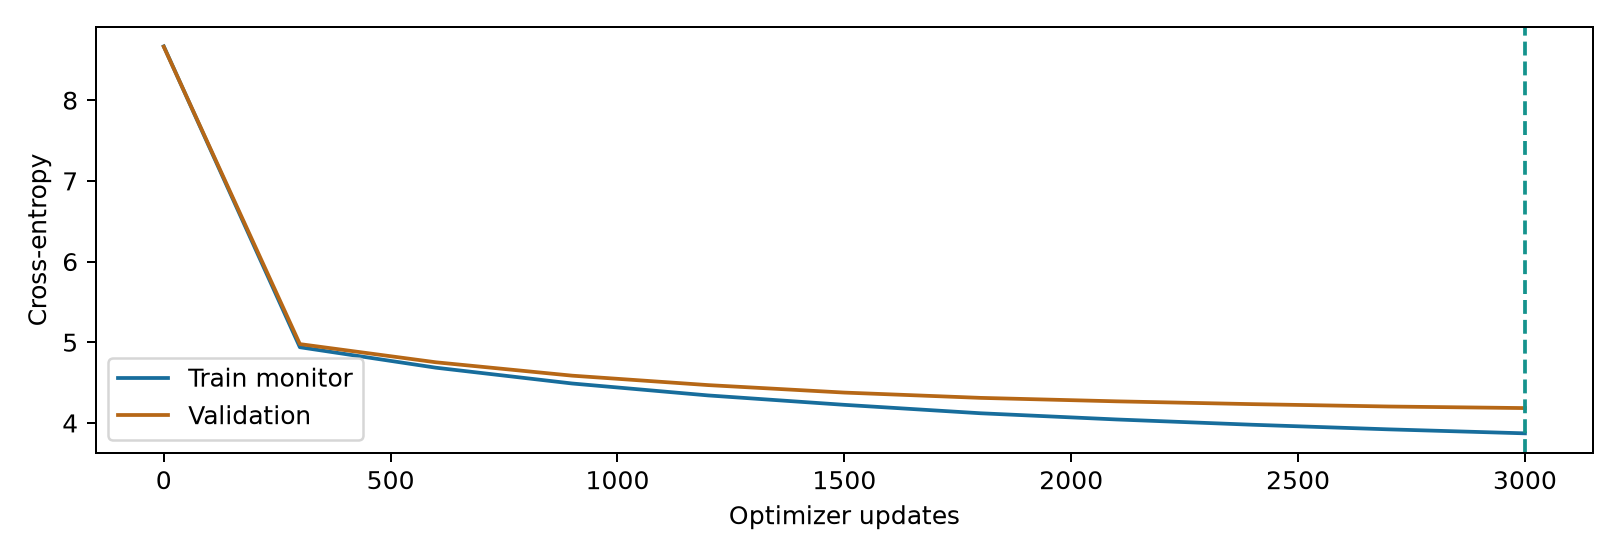
\includegraphics[width=.96\linewidth]{assets/reference-loss.png}
\end{center}
横轴是更新次数，纵轴是每字符交叉熵；训练监测使用训练文本前8193字符，验证遍历完整验证集。本次最低验证损失4.184194出现在预算末尾3000步，曲线末段仍在下降；最佳训练时长还需结合后续验证曲线判断。

选定权重测试交叉熵4.177170、困惑度65.18；同一目标上的加一平滑二元基线困惑度338.35。测试计分142420字符，原始未知字符210个。困惑度比较使用相同的数据与词表。
\begin{examplebox}[原样输出首段：温度0.8，种子2026，开头“春”]
\begin{center}\large
春梦满江南，\\
秋风吹赤城。\\
露下高秋水，\\
烟霞湿牛歌。
\end{center}
四句五字的形式已经出现，但“烟霞湿牛歌”等搭配不自然。这是单次采样的输出，生成稳定性由下面的批量采样统计分析。
\end{examplebox}
固定开头“春、山、月、江、秋”，每个温度每个开头批量采样20份，共100份；只评价未经修改的首段。温度0.6、0.8、1.0、1.2下四句五言比例分别为55\%、72\%、79\%、78\%。贪心仅采5份，四句五言0/5。这些样本未检出整首训练诗复现；该检查覆盖完全重合，近似改写与原创性需另行分析。

旧小语料的无衰减10万步模型，温度0.8下虽有70/100份满足结构，但51/100份整首复现训练诗。本次两组长训练均未观察到典型grokking（延迟泛化跃迁），这一观察对应当前语料、预算与训练设置。课堂应同时分析验证损失、结构、语义和训练文本重合。

\clearpage
\section{评估、报告与课程接口}
\subsection{一次最终测试}
在验证集确定方案之后，使用同一选定目录提交：
\begin{lstlisting}[language=bash]
bash scripts/submit.sh evaluate
\end{lstlisting}
网页提交时保留资源、解释器、数据及选定运行目录设置，末行改为\file{bash scripts/run-job.sh evaluate}。
结果存入\texttt{\detokenize{outputs/evaluate-作业号/test_metrics.json}}。报告神经网络与二元字符计数基线的测试交叉熵和困惑度；两者在相同目标字符上评分。二元基线只根据前一个字符预测，使用训练相邻字符计数及加一平滑：
\begin{equation}
p(v\mid u)=\frac{C_{uv}+1}{\sum_{r=0}^{V-1}C_{ur}+V}.
\end{equation}
$C_{uv}$是训练中字符$u$后紧接$v$的次数。平滑避免未见字符对概率为0。基线结果对应本次加一平滑二元模型的设置。
\subsection{指标、泛化与任务代价}
交叉熵衡量对真实下一字赋予的概率；困惑度只能在相同词表、数据和计分协议下比较。未知字符统一映射为同一词元，报告中同时列出其数量，比较时保持词表一致。准确率容易被标点和常见字主导，因此本实验以交叉熵和原始生成分析为主。

工作流为：明确古诗续写任务与展示目标，确定数据来源，整首去重和划分，训练集建立词表，设计因果模型及损失，优化并用验证集选择，最后测试与生成；后续监测输入中未见字、重复与内容偏移。本实验分别评价诗歌格式、语义与训练文本重合；原创性、事实正确性和通用问答能力各有不同的评估要求。
\subsection{评分与提交}
\par\noindent\begin{tabularx}{\linewidth}{L{4cm}L{1.5cm}Y}\toprule
部分 & 分值 & 可观察证据\\\midrule
目标、维度与推导 & 15 & 输入标签、形状、注意力手算\\
T1--T4实现 & 35 & 错位标签、拆合头、掩码、残差\\
T5--T6与自检 & 25 & 模型、损失、因果性、更新、生成\\
训练与生成对照 & 15 & 验证选择、四份原文、基线\\
复现与分析 & 10 & 作业记录、配置、误差与局限\\\bottomrule
\end{tabularx}\par
提交\texttt{\detokenize{学号_姓名_lab06.zip}}：代码、\file{report.pdf}、选定训练目录（含权重与代码快照）、四份生成及参数、一次测试结果、Slurm日志和作业状态。去掉缓存、环境和重复数据；保留来源与指纹。
\subsection{课后练习与下次接口}
必答：解释未来信息泄漏、拆头的轴顺序、训练和生成前缀差异。选做只改变层数、上下文或位置参数之一，固定其他条件，在验证集讨论效果和代价，最后用测试集评价选定方案。下一次将同一个“数据—目标—模型—优化—评估”流程用于理解预训练与微调；本实验只实现了其中的小规模自回归训练。

\clearpage
\section{符号索引与资料来源}
\subsection{符号按角色索引}
\par\noindent\begin{tabularx}{\linewidth}{L{2.7cm}Y L{1.9cm}}\toprule
类别与符号 & 含义 & 首次解释\\\midrule
数据：$n,B,T,V$ & 样本编号、批量、序列长度、词表大小 & 2.1--2.2\\
$\mathbf x^{(n)},\mathbf y^{(n)}$ & 长$T$整数输入、标签；括号上标只表示样本 & 2.2\\
模型：$d,H,k,L,\ell$ & 表示宽度、头数、头宽、块数、层编号 & 3.1、4.1\\
$\mathbf A_\ell^{(n)}$ & 单样本逐位置表示，$T\times d$ & 4.1\\
$\mathbf Q,\mathbf K,\mathbf V$ & 单头查询、键、值，$T\times k$ & 3.1\\
$\mathbf S,\mathbf M,\mathbf P$ & 分数、掩码、注意力权重，$T\times T$ & 3.2\\
$\mathbf O$ & 单头加权输出，$T\times k$ & 3.2\\
概率：$\theta,p_\theta,\mathbf z$ & 参数集合、条件概率、词表原始得分 & 5.1--5.2\\
$\mathcal L^{(n)},\mathcal L_B$ & 单样本与批量平均交叉熵 & 5.1\\
$\tau,C_{uv}$ & 采样温度、训练相邻字符对计数 & 7.1、8.1\\
算子：$\top,\sum,\prod$ & 转置、求和、连乘 & 3.1--3.2、5.1\\
$\exp,\log,\partial$ & 指数、自然对数、偏导 & 3.2、5.1--5.2\\\bottomrule
\end{tabularx}\par

\subsection{实际使用的资料及改编边界}
\begin{enumerate}[leftmargin=1.5em,itemsep=.2em]
\item \texttt{\detokenize{教案/人工智能数学原理与算法_12次课程与助教分工_最终版.xlsx}}，第7--9次：注意力、Transformer、预训练。实验课时沿用实验五。
\item \file{source/pdf/nndl-v2.pdf}，邱锡鹏《神经网络与深度学习》，8.4.3--8.4.4与13.1--13.1.1；已核对文件第246--247、375--376页。教材词元按列排列，本讲义改为位置按行，样本单列批量轴。
\item \texttt{\detokenize{教案/第八次教学_Transformer/sections/05_decoder.tex}}，因果掩码、右移目标、教师强制；保留课程记号。手算分数与热身是教学设定。
\item \href{https://github.com/OthersideAI/tinyGPT}{OthersideAI/tinyGPT}，版本\file{e8564668}：模型、采样与字符接口；附版权许可。该仓库由OthersideAI维护，是minGPT的分叉。
\item \href{https://github.com/karpathy/minGPT}{Karpathy/minGPT}与\href{https://github.com/karpathy/nanoGPT}{nanoGPT}：作者的教学与训练参考。输入输出嵌入不共享，优化调度在课堂版简化。
\item \href{https://isaacperez.github.io/posts/TinyGPT/}{Isaac Pérez：TinyGPT}及其原始仓库：纯Python、零依赖框架的教学定位，作为扩展阅读。本课107训练运行PyTorch实现。
\item \href{https://goclawai.cn/llm/start/}{GoClaw导学}与\href{https://goclawai.cn/llm/tiny-gpt/}{从零训练TinyGPT}：短作业、训练重载与对照活动设计。
\item \href{https://github.com/THUNLP-AIPoet/Datasets/tree/master/CCPC}{THU-CCPC}，固定版本\file{0a53d6a2}：本次五言诗正文；仅供学术使用，引用Guo等2019年Jiuge论文。旧chinese-poetry小语料仅作历史对照。
\item 《坑 of 本科生算力平台.docx》：文件上传、环境路径与网页界面；作业提交与清屏命令分别参见\href{https://slurm.schedmd.com/sbatch.html}{Slurm文档}与\href{https://invisible-island.net/ncurses/man/clear.1.html}{clear手册}。QOS按账号可用项填写。
\end{enumerate}
\end{document}

